\documentclass[12pt,a4paper]{article}
\usepackage[utf8]{inputenc}
\usepackage[T1]{fontenc}
\usepackage[italian]{babel}

\usepackage{verbatim}

\begin{comment}
\addto\captionsitalian{%
  \renewcommand{\abstractname}{Abstract}%
}
\end{comment}

\usepackage{subcaption}
\usepackage{graphicx}
\usepackage{fancyhdr}
\usepackage{titlesec}
\usepackage{lmodern}
\usepackage{geometry}
\usepackage{setspace}
\usepackage{parskip}
\usepackage{listings}
\usepackage{xcolor}
\usepackage{enumitem}
\usepackage{float}
\usepackage{booktabs}
\usepackage{csquotes}
\usepackage{tabularx} 

\usepackage[
    backend=biber,
    style=numeric,
    sorting=none
]{biblatex}
\addbibresource{riferimenti.bib}

\usepackage{hyperref}
\hypersetup{colorlinks=true, linkcolor=blue, citecolor=blue, urlcolor=blue}
\usepackage{xurl}

\addtolength{\skip\footins}{1cm}

\definecolor{codegreen}{rgb}{0,0.6,0}
\definecolor{codeblue}{rgb}{0.2,0.2,0.7}
\definecolor{backcolor}{rgb}{0.95,0.95,0.90}

\lstdefinestyle{mystyle}{
    backgroundcolor=\color{backcolor},   
    commentstyle=\color{codegreen}\itshape,
    keywordstyle=\color{blue},
    numberstyle=\tiny\color{black},
    stringstyle=\color{codegreen},
    basicstyle=\ttfamily\footnotesize,
    breaklines=true,
    captionpos=b,
    keepspaces=true,
    numbers=left,
    numbersep=8pt,
    showspaces=false,
    showstringspaces=false,
    showtabs=false,
    frame=shadowbox,
    language=Python
}

\lstset{style=mystyle}

\geometry{top=2.5cm,bottom=2.5cm,left=2.5cm,right=2.5cm}

% --- CONFIGURAZIONE LISTINGS PER JAVASCRIPT ---
\definecolor{lightgray}{rgb}{.95,.95,.95}
\definecolor{darkgray}{rgb}{.4,.4,.4}
\definecolor{purple}{rgb}{0.65, 0.12, 0.82}

\lstdefinelanguage{JavaScript}{
  keywords={break, case, catch, continue, debugger, default, delete, do, else, false, finally, for, function, if, in, instanceof, new, null, return, switch, this, throw, true, try, typeof, var, void, while, with, const, let},
  morecomment=[l]{//},
  morecomment=[s]{/*}{*/},
  morestring=[b]',
  morestring=[b]",
  ndkeywords={class, export, boolean, throw, implements, import, this},
  keywordstyle=\color{blue}\bfseries,
  ndkeywordstyle=\color{darkgray}\bfseries,
  identifierstyle=\color{black},
  commentstyle=\color{purple}\ttfamily,
  stringstyle=\color{codegreen}\ttfamily,
  sensitive=true
}

\lstdefinelanguage{Dart}{
  keywords={abstract, as, assert, async, await, break, case, catch, class, const, continue, default, deferred, do, dynamic, else, enum, export, extends, extension, external, factory, false, final, finally, for, Function, get, hide, if, implements, import, in, is, late, library, mixin, new, null, on, operator, part, required, rethrow, return, set, show, static, super, switch, sync, this, throw, true, try, typedef, var, void, while, with, yield},
  morecomment=[l]{//},
  morecomment=[s]{/*}{*/},
  morestring=[b]',
  morestring=[b]",
  keywordstyle=\color{blue}\bfseries,
  identifierstyle=\color{black},
  commentstyle=\color{codegreen}\ttfamily,
  stringstyle=\color{codegreen}\ttfamily,
  sensitive=true
}

\lstset{
    style=mystyle,
    language=JavaScript,
    breaklines=true,
    postbreak=\mbox{\textcolor{red}{$\hookrightarrow$}\space},
}


\begin{document}

\begin{titlepage}
    \centering
    \vspace*{1.5cm}
    {\scshape\LARGE Università degli Studi di Udine \par}
    \vspace{0.4cm}
    {\scshape\Large Dipartimento di Scienze Matematiche, Informatiche e Fisiche\par}
    \vspace{0.4cm}
    {\large IBML - Internet of Things, Big Data, Machine Learning \par}
    \vspace{0.4cm}
    \vspace{1.5cm}
    
\includegraphics[width=0.25\textwidth]{immagini/Logo.pdf}\par
    \vspace{1cm}
    \rule{\textwidth}{0.5pt}\vspace{0.4cm}
    {\bfseries\LARGE Internet of Things\\[0.2cm]
    Progetto Pet Tracker \par}
    \rule{\textwidth}{0.5pt}
    \vfill
    \begin{flushleft}
    \textit{\textbf{Autori}}\\
    Andrea Gioia, 169484 \hfill 169484@spes.uniud.it \\
    Alessio Nicodemo, 166972 \hfill 166972@spes.uniud.it \\
    Mattia Nadal,  167372\hfill 167372@spes.uniud.it \\
    Francesco Sabot, 167339  \hfill 167339@spes.uniud.it
    \end{flushleft}
\end{titlepage}

\begin{abstract}

\noindent 
Il progetto Pet Tracker propone la realizzazione di un sistema 
per il tracciamento in tempo reale di animali domestici di taglia media o grande, 
tramite un dispositivo \textit{embedded} indossabile.
L'obiettivo del lavoro è sviluppare una soluzione affidabile, 
scalabile e a basso consumo per il monitoraggio continuo dell'animale. \\

\noindent
La soluzione si basa su una piattaforma
ESP32-S3 con connettività LTE e modulo GNSS, 
in grado di acquisire e trasmettere 
lo stato della batteria del dispositivo, 
insieme alla posizione geografica e 
all'attività motoria dell'animale, 
verso un \textit{backend} remoto.
L'architettura del sistema segue il modello \textit{IoT World Forum} (IoTWF)
e integra diverse tecniche di ottimizzazione energetica, 
tra cui l'utilizzo delle modalità \textit{deep sleep} e \textit{hot start}. 
I dati raccolti vengono elaborati dal \textit{backend}, resi accessibili tramite API REST 
e visualizzati attraverso un'applicazione mobile dedicata. 

\end{abstract}

\newpage

\tableofcontents

\newpage

\begin{comment}
\section{Architettura del sistema}

L'architettura del sistema Pet Tracker segue il modello a sette livelli dell'IoTWF, 
garantendo una transizione strutturata dal dato fisico all'informazione per l'utente.

\subsection{Mappatura sul modello IoTWF}

\begin{itemize}
    \item \textbf{Livello 1 (Physical Devices):} microcontrollore, sensori e batteria.
    \item \textbf{Livello 2 (Connectivity):} modem LTE e protocolli di comunicazione sicuri.
    \item \textbf{Livello 3 (Edge Computing):} elaborazione locale sul microcontrollore per il filtraggio delle stringhe NMEA e il calcolo dei passi.
    \item \textbf{Livello 4 (Data Accumulation):} persistenza dei dati sul server PocketBase basato su database SQLite.
    \item \textbf{Livello 5 (Data Abstraction):} pubblicazione dei dati tramite API REST in formato JSON.
    \item \textbf{Livello 6 (Application):} applicazione mobile per la visualizzazione delle informazioni e della posizione dell'animale su mappa.
    \item \textbf{Livello 7 (Collaboration and Processes):} interazione dell'utente con il sistema per il monitoraggio dell'animale.
\end{itemize}
\end{comment}

\section{Hardware}

\subsection{LilyGo T-SIM7670G-S3}

Il dispositivo utilizza una scheda LilyGo T-SIM7670G-S3 \cite{lilygo_specs} basata sul microcontrollore ESP32-S3 dual-core.
Quest'ultimo gestisce la logica applicativa e la comunicazione con il modem SIM7670G tramite interfaccia UART.

\subsection{Antenne LTE e GNSS}

Il sistema utilizza un'antenna flessibile LTE \cite{LTE} per la connettività dati e un'antenna ceramica attiva \cite{GPS} per il ricevitore GNSS integrato, volta a garantire la precisione della localizzazione \textit{outdoor}.

\subsection{Batteria e power Management}

Il sistema è alimentato da una batteria ricaricabile agli ioni di litio da 3000~mAh e 30~A. Il monitoraggio della carica avviene tramite un partitore di tensione collegato al pin \texttt{ADC\_BAT} (GPIO 4), per calcolarne la percentuale residua.

\subsection{BMA400 CJMCU-400}

L'accelerometro utilizzato è un BMA400 \cite{bma400} integrato sulla \textit{breakout board} CJMCU-400. Il sensore viene interrogato per rilevare il movimento, consentendo l'implementazione di un contapassi utile al monitoraggio dell'attività motoria dell'animale.

\section{Firmware: logica di funzionamento}

Il firmware, sviluppato in ambiente Arduino per 
il \textit{System on Chip} (SoC) ESP32-S3, 
gestisce l'acquisizione dei dati dai sensori, 
il controllo del modem LTE e l'ottimizzazione energetica 
tramite una macchina a stati finiti.

\subsection{Gestione della persistenza e hot start}

Per ridurre drasticamente il \textit{Time To First Fix} (TTFF) del modulo GNSS, il firmware
sfrutta la memoria \textit{Real-Time Clock} (RTC) dell'ESP32. 
Tale area di memoria consente di preservare i dati critici 
anche durante i cicli di \textit{deep sleep}. 
Le variabili critiche, come l'ultima posizione valida 
(\texttt{lastLat}, \texttt{lastLon}) e i timestamp
(\texttt{lastGpsDate}, \texttt{lastGpsTime}), 
vengono dichiarate con l'attributo \texttt{RTC\_DATA\_ATTR}.

Al risveglio del dispositivo, la funzione \texttt{iniettaGps()} esegue le seguenti operazioni:
\begin{itemize}
    \item Recupera le coordinate geografiche e temporali salvate nel ciclo precedente;
    \item Inietta la posizione nota nel modulo GNSS tramite il comando \texttt{AT+CGNSSPOS};
    \item Sincronizza l'orario del modem con il comando \texttt{AT+CGNSSTIME}.
\end{itemize}

Questo meccanismo abilita la modalità \textit{hot start}, che minimizza il tempo di ricerca dei
satelliti e, di conseguenza, il consumo energetico del sistema.

\subsection{Protocollo di comunicazione HTTPS}

La trasmissione dei dati al \textit{backend} PocketBase è affidata a una serie di comandi AT inviati
via seriale al modem SIM7670G. Il firmware incapsula le informazioni in un oggetto JSON
strutturato, trasmesso tramite una richiesta HTTPS POST. Il \textit{payload} include:

\begin{itemize}
    \item \texttt{board\_id}: un identificativo univoco derivato dall'IMEI del modem;
    \item \texttt{geo}: un oggetto con latitudine e longitudine per la gestione cartografica;
    \item \texttt{battery} / \texttt{battery\_percent} / \texttt{charging}:
          parametri relativi allo stato di carica della batteria;
    \item \texttt{steps}: conteggio dei passi rilevato dall'accelerometro nella sessione corrente;
    \item \texttt{sleep}: flag booleano che segnala al server l'imminente entrata in stato
          di inattività;
    \item \texttt{trip}: flag booleano che segnala al server che l'animale si trova su un
          veicolo in movimento. Quando attivo, ha priorità assoluta sulla logica di \textit{geofencing}
          e sopprime il \textit{deep sleep} per garantire la continuità del tracciamento.
\end{itemize}

La sequenza di invio si avvale dei comandi \texttt{AT+HTTPINIT}, \texttt{AT+HTTPPARA}
e \texttt{AT+HTTPDATA} per configurare la sessione HTTP, inserire i dati e infine avviare
la trasmissione con \texttt{AT+HTTPACTION=1}. Al termine di ogni invio, la sessione viene
chiusa con \texttt{AT+HTTPTERM} per liberare le risorse del modem.

\subsection{Risparmio energetico}

Per massimizzare l'autonomia, la gestione energetica 
viene modulata in base alla rilevazione del movimento e allo stato di viaggio:

\begin{enumerate}
    \item \textbf{Rilevamento Attività:} il firmware monitora costantemente il numero di passi,
          azzerando a ogni nuovo movimento un timer di inattività (\texttt{lastActivityTime}).
    \item \textbf{Modalità Viaggio:} se il flag \texttt{trip} è attivo (velocità GPS $>$ 10\,km/h), 
          il \textit{deep sleep} viene disabilitato indipendentemente dall'inattività rilevata
          dall'accelerometro, garantendo la trasmissione dei dati a intervalli regolari durante il viaggio.
    \item \textbf{Ibernazione:} se non viene rilevata attività per un tempo superiore a
          \texttt{SLEEP\_TIMEOUT} (30~secondi) e il flag \texttt{trip} non è attivo, il sistema
          invia un ultimo pacchetto dati aggiornando il flag \texttt{sleep} a \texttt{true}, entrando in \textit{deep sleep}. 
          Vengono quindi spenti i moduli radio tramite i comandi \texttt{AT+CGNSSPWR=0} e \texttt{AT+CPOWD=1}. Il risveglio
          è gestito tramite interrupt hardware sul pin \texttt{GPIO\_5}, generato dall'accelerometro
          solo al rilevamento di un nuovo movimento.
\end{enumerate}

Inoltre, il firmware integra specifiche strategie di controllo energetico 
volte a eliminare i consumi statici e a prevenire alterazioni nelle letture dei sensori:

\begin{itemize}
    \item \textbf{Controllo ADC:} il circuito del partitore di tensione per la batteria viene
          attivato solo durante la lettura tramite il pin \texttt{BAT\_ADC\_EN}, garantendo la
          precisione del voltaggio acquisito dal pin \texttt{ADC\_BAT}. Il valore grezzo viene
          mediato su 10 campionamenti consecutivi e scalato con fattore pari a 2 per compensare il partitore. 
          La percentuale di carica è calcolata per interpolazione lineare
          nell'intervallo compreso tra 3,4~V e 4,2~V,
          corrispondenti rispettivamente a 0\% e a 100\% di carica.
    \item \textbf{Stato USB:} dal registro hardware \texttt{USB\_SERIAL\_JTAG\_\allowbreak EP1\_CONF\_REG} dell'ESP32, 
          il sistema rileva se il dispositivo è collegato a una fonte di ricarica USB, impostando
          dinamicamente il campo \texttt{charging} nel pacchetto dati. In stato di ricarica,
          tensione e percentuale non vengono aggiornate per evitare misurazioni alterate dalla
          corrente in ingresso, vengono invece restituiti gli ultimi dati validi salvati nella memoria RTC.
\end{itemize}

\subsection{Acquisizione GPS e timeout}

Il modulo GNSS viene interrogato tramite il comando \texttt{AT+CGNSSINFO}.
La risposta viene analizzata campo per campo, estraendo latitudine, longitudine e velocità
in formato decimale, evitando la necessità di conversione dal formato NMEA gradi-minuti.
Il firmware attende fino a un massimo di \texttt{GPS\_TIMEOUT} (180~secondi) per ottenere
un fix valido; superato tale limite senza una posizione acquisita, il ciclo corrente viene
saltato e il sistema ritenta al loop successivo. Una volta ottenuto un fix valido, le
coordinate e il timestamp vengono salvati in memoria RTC per abilitare l'\textit{hot start} al
ciclo successivo.

\subsection{Connessione alla rete LTE}

All'avvio, il firmware tenta di registrarsi alla rete LTE attraverso la funzione
\path{connectToNetworkFast()}. Vengono configurati la modalità radio
(\texttt{AT+CNMP=38} per LTE only), il profilo APN dell'operatore e l'attivazione del
contesto dati con \texttt{AT+CNACT=0,1}. La registrazione viene verificata in polling
tramite il comando \texttt{AT+CEREG?}, controllando la presenza dei codici di stato
\texttt{0,1} (registrato in rete home) o \texttt{0,5} (roaming). Se entro
\texttt{NET\_TIMEOUT} (60~secondi) la registrazione non viene completata, il dispositivo
entra direttamente in \textit{deep sleep} per evitare consumi inutili in assenza di copertura.

\section{Backend e database}

La gestione della persistenza e della modellazione dei dati è basata su PocketBase \cite{pocketbase},
una soluzione open-source strutturata su SQLite scelta per la sua reattività, 
il ridotto consumo di risorse e il supporto di un'interfaccia API RESTful. 
La logica applicativa lato server e l'integrazione dei flussi di dati si sviluppano estendendo 
il nucleo del framework direttamente nel file principale di runtime \texttt{main.pb.js}, 
che gestisce sia gli eventi reattivi, noti come \textit{hooks}, sia i servizi temporali pianificati, definiti \textit{cron jobs}.
Poiché il runtime JavaScript di PocketBase si basa sull'interprete Goja incorporato in Go, 
l'intera esecuzione del codice avviene in modalità \textit{single-threaded}, 
condividendo il medesimo spazio d'esecuzione globale e lo stesso ciclo di eventi del server.

\subsection{Architettura di hosting e operational continuity}
La gestione operativa dell'infrastruttura di backend è stata ottimizzata per garantire la disponibilità del dato, la tolleranza ai guasti e il monitoraggio dei flussi durante la fase di prototipazione e test:
\begin{itemize}
    \item \textbf{Network Exposure (NAT Traversal):} l'istanza è ospitata su una \textit{workstation locale} e data la necessità di connettersi al backend sia dal dispositivo (tramite rete cellulare LTE) sia dall'applicazione mobile (tramite rete dati/Wi-Fi), il vincolo del \textit{NAT Traversal} e l'assenza di un IP pubblico statico sulla rete locale sono stati superati mediante l'impiego di ngrok \cite{ngrok}. Questa tecnologia di \textit{tunneling} crea un canale sicuro HTTPS fungendo da \textit{reverse proxy}, reindirizzando il traffico in ingresso verso l'istanza locale di PocketBase e garantendo l'accessibilità dei servizi in tempo reale.
    \item \textbf{Strategia di Backup a Caldo (Data Retention):} per garantire la resilienza dei dati e prevenire perdite accidentali dovute a guasti del server locale, è stato strutturato un sistema di backup automatizzato tramite l'utility rclone \cite{rclone}, uno strumento a riga di comando per la gestione del cloud storage. Il processo è configurato per eseguire la sincronizzazione incrementale della directory dei dati di PocketBase verso un \textit{bucket remoto} su Backblaze B2 \cite{backblaze} tramite un \textit{cron job} a cadenza mensile.    
    \item \textbf{Monitoraggio Esterno e Uptime:} l'accessibilità e lo stato di salute del sistema sono vigilati esternamente tramite UptimeRobot \cite{uptimerobot}. Dato che l'accessibilità del backend dipende dalla stabilità del tunnel ngrok, il monitoraggio interroga l'endpoint HTTPS a intervalli regolari, isolando tempestivamente le anomalie di rete e inviando notifiche immediate in caso di interruzione del tunnel o del server locale.
\end{itemize}
\subsection{Modellazione dei dati e API rules}
I dati inviati dalla board transitano nella collezione di staging \texttt{data\_sent\_raw}, la quale funge da punto di ingresso grezzo ed isola il database da potenziali fluttuazioni della rete cellulare. La struttura del record prevede i seguenti campi tipizzati:
 
\begin{itemize}
    \item \texttt{timestamp}: Riferimento temporale hardware dell'acquisizione.
    \item \texttt{lat} / \texttt{lon}: Coordinate geografiche acquisite dal modulo GNSS.
    \item \texttt{battery} / \texttt{battery\_percent}: Stato di carica dell'accumulatore espresso in voltaggio e percentuale.
    \item \texttt{charging}: Variabile booleana indicante se la batteria è in corso di ricarica.
    \item \texttt{steps}: Conteggio lineare dei passi rilevato dall'accelerometro BMA400.
    \item \texttt{sleep}: Flag booleano indicante se il dispositivo è in stato di \textit{deep sleep}.
    \item \texttt{trip}: Flag booleano indicante se l'animale si trova su un veicolo in movimento.
\end{itemize}
L'accesso alle collezioni memorizzate nel backend avviene esclusivamente tramite l'interfaccia RESTful API fornita nativamente, separando nettamente il livello di persistenza dal livello di fruizione mobile dell'applicazione Flutter. 

\begin{comment}
L'integrità e la riservatezza delle informazioni sono rigidamente normate da \textbf{API Rules} basate su espressioni booleane che implementano il principio del minimo privilegio:
\begin{itemize}
    \item \textbf{List/View:} Visualizzazione e interrogazione dei record permesse esclusivamente agli utenti client preventivamente autenticati.
    \item \textbf{Create:} Abilitata per la board LilyGo tramite un account di autenticazione dedicato al dispositivo edge.
    \item \textbf{Update/Delete:} Operazioni distruttive o di modifica strutturale ristrette ai soli amministratori del sistema (\textit{Admin Only}).
\end{itemize}
\end{comment}

\subsection{Pulizia e Normalizzazione (Server-side Hooks)}
L'elaborazione dei messaggi IoT segue un pattern \textit{Staging-and-Purge} sequenziale gestito lato server tramite i \textit{JavaScript Event Hooks} nativi del sistema. L'hook \path{onRecordAfterCreateSuccess} si attiva immediatamente dopo il consolidamento con successo di ogni pacchetto grezzo nella collezione \texttt{data\_sent\_raw}. 
Per ottimizzare le performance computazionali ed eliminare query ridondanti nello stesso ciclo, il sistema esegue una \textbf{lettura centralizzata} della configurazione della scheda (\texttt{getBoardRecord}) all'inizio dell'esecuzione dell'hook, distribuendo il record ottenuto come parametro a tutte le funzioni della pipeline. Il trigger elabora ogni pacchetto in quattro fasi sequenziali:
\begin{enumerate}
    \item \textbf{Batteria:} Salva il record nella collezione verticale \texttt{battery\_data} e verifica se inviare notifiche push di cambio soglia o allerta energetica.
    \item \textbf{Activity Tracking:} Delega l'analisi della telemetria al modulo \path{activity\_manager.js}, che aggiorna la macchina a stati e gestisce la persistenza delle sessioni.
    \item \textbf{Posizioni:} Salva le coordinate GPS nella collezione \texttt{positions} agganciandole all'attività determinata al punto precedente, a condizione che i dati GNSS siano validi e l'attività non sia stata rigettata.
    \item \textbf{Eliminazione dato grezzo:} Rimuove permanentemente il record originario da \texttt{data\_sent\_raw} all'interno del blocco \texttt{finally} dell'hook. Questo costrutto non serve a garantire l'atomicità transazionale (poiché l'evento scatta a inserimento già consolidato), ma funge da garante di svincolo per l'ottimizzazione dello spazio fisico: assicura la cancellazione fisica del record di staging e previene il rigonfiamento del database SQLite anche qualora una delle funzioni logiche precedenti (es. il modulo attività o il salvataggio della posizione) dovesse lanciare un'eccezione non gestita a runtime.
\end{enumerate}
\subsection{Macchina a Stati delle Attività e Logiche di Isteresi}
Il cuore del modulo \texttt{activity\_manager.js} è una macchina a stati che modella il comportamento cinematico e geografico dell'animale. Gli stati sono suddivisi in \textit{attivi} (dispositivo sveglio) e \textit{sleep} (dispositivo in \textit{deep sleep}), legati da una corrispondenza biunivoca riassunta nella Tabella~\ref{tab:stati}.
\begin{table}[H]
\centering
\small
\begin{tabularx}{\textwidth}{m{2.3cm}m{2.1cm}ccX}
\toprule
\textbf{Attivi} & \textbf{Sleep} & \textbf{Allarme} & \textbf{Geofence} & \textbf{Descrizione} \\ \midrule
\texttt{i} (inside)   & \texttt{d}           & Any                     & True              & Animale all'interno del perimetro sicuro. \\
\texttt{v} (trip) & \texttt{a}           & False                   & False             & In viaggio su veicolo, allarme spento. \\ 
\texttt{r} (trip)  & \texttt{q}           & True                    & False             & In viaggio su veicolo, allarme attivo (critico). \\
\texttt{w} (walk)     & \texttt{z}           & False                   & False             & Fuori perimetro in passeggiata, allarme spento. \\
\texttt{s} (search)   & \texttt{p}           & True                    & False             & Fuori perimetro, allarme attivo (emergenza). \\ \bottomrule
\end{tabularx}
\caption{Macchina a stati delle attività: corrispondenze tra stati attivi e sleep.}
\label{tab:stati}
\end{table}
Tutti gli stati sleep si comportano in modo uniforme: vengono sempre archiviati come sessioni storiche chiuse impostando il flag \texttt{is\_active = false}. Prima di eseguire qualsiasi valutazione di business logic, la funzione \texttt{computeStatus} normalizza internamente gli stati sleep convertendoli nel rispettivo equivalente attivo (tramite il dizionario \texttt{SLEEP\_TO\_ACTIVE}, es. \texttt{"a"} $\to$ \texttt{"v"} e \texttt{"q"} $\to$ \texttt{"r"}). Questo garantisce che la logica di analisi riconosca da quale contesto provenga l'animale anche dopo lunghe fasi di inattività hardware.
Al fine di minimizzare la granularità dei record sul DBMS e ottimizzare le query storiche, il sistema applica un principio di \textbf{estensione temporale}: se un pacchetto conferma lo stato corrente, l'activity manager si limita ad aggiornare il timestamp di fine evento (\texttt{end\_time}) e a incrementare il contatore lineare dei passi (\texttt{total\_steps}). La creazione di una nuova riga nel database (con la contestuale chiusura permanente della precedente) avviene esclusivamente in presenza di un'effettiva transizione di stato. Una transizione tra \texttt{"v"} e \texttt{"r"} indotta dal cambio manuale del flag di allarme da parte dell'utente forza la chiusura e la riapertura immediata della sessione, garantendo la tracciabilità del cambio di contesto e la variazione del livello di urgenza delle notifiche.
Le transizioni tra gli stati sono governate da un algoritmo a priorità decrescente:
\begin{enumerate}
    \item \textbf{Priorità 1 (Massima) - Stato Viaggio:} Se il flag \texttt{trip = true} e il contatore dei passi è nullo (\texttt{steps == 0}), lo stato viene forzato a \texttt{"v"} o \texttt{"r"} a seconda dell'allarme, azzerando i falsi positivi derivanti da movimenti muscolari isolati dell'animale o rumore dell'accelerometro.
    \item \textbf{Priorità 2 - Memoria del Viaggio:} Qualora il sensore hardware rilevi il termine del viaggio (\texttt{trip = false}) ma l'animale non ha ancora computato passi (\texttt{steps == 0}), il sistema applica una memoria di stato: assume che il veicolo sia momentaneamente fermo (es. a un semaforo o in sosta con l'animale a bordo) e preserva lo stato \textit{Trip} corrente (\texttt{"v"} o \texttt{"r"}). Il ricalcolo geografico pulito si attiva solo se \texttt{steps > 0}, ovvero al primo movimento muscolare effettivo.
    \item \textbf{Priorità 3 - Analisi Geofence:} Se l'animale si trova all'interno delle coordinate del cerchio sicuro configurato, lo stato viene impostato a \texttt{"i"} (Inside).
    \item \textbf{Priorità 4 (Minima) - Stato Esterno:} Analisi combinata delle coordinate esterne e dell'allarme utente, che determina la transizione in passeggiata ordinaria (\texttt{"w"}) o nello stato critico di ricerca (\texttt{"s"}).
\end{enumerate}

\subsection{Lifecycle del deep sleep e servizi temporali}
\subsubsection{Gestione del risveglio e anti-spuria}
Al risveglio dal \textit{deep sleep}, il tracker trasmette un pacchetto privo di una sessione attiva aperta sul database, in quanto la precedente era stata chiusa all'atto dell'addormentamento. Il sistema interroga la collezione escludendo i record anomali ed estrae la sessione chiusa più recente (\texttt{recentClosed}) per ricavare il \texttt{prevStatus} corretto da passare a \texttt{computeStatus}.

Il sistema gestisce il risveglio secondo due scenari logici:
\begin{itemize}
    \item \textbf{Risveglio nello stesso stato:} Se lo stato attivo calcolato coincide con lo stato attivo di partenza dello sleep precedente (es. dormiva in casa \texttt{"d"} normalizzato a \texttt{"i"}, e il nuovo stato è ancora \texttt{"i"}), la sessione viene riattivata in continuità impostando \texttt{is\_active = true} senza limiti temporali, evitando frammentazioni e collegando le attività attraverso i cicli di sonno.
    \item \textbf{Risveglio con cambio di stato:} La sessione chiusa viene sanata convertendo lo status nella sua versione attiva originaria a fini di coerenza storica (es. \texttt{"d"} $\to$ \texttt{"i"}), e viene parallelamente istanziata una nuova attività con il nuovo stato calcolato. Le sessioni chiuse dal watchdog con \texttt{anomaly = true} sono tassativamente escluse da questo flusso e non vengono mai riattivate.
\end{itemize}
Per ottimizzare l'efficienza del thread unico di esecuzione, il modulo implementa un \textbf{filtraggio delle notifiche spurie} (\textit{STEP 3 anticipato}): se viene ricevuto un pacchetto di quiete (\texttt{sleep=true}) in assenza di una sessione attiva sul database, l'inserimento viene intercettato e scartato preventivamente a livello logico, impedendo la proliferazione di record ridondanti e l'invio di catene di notifiche push duplicate all'utente.
\subsubsection{Watchdog di Inattività e Split Notturno}
La coerenza temporale delle sessioni e l'allineamento dei calendari storici sono garantite da due cron job registrati all'avvio nel thread principale dell'applicazione:
\begin{itemize}
    \item \textbf{Watchdog (ogni minuto):} Isola le sessioni attive che non trasmettono dati entro un intervallo stabilito (10 minuti), causate da anomalie impreviste (es. perdita di segnale LTE o spegnimento repentino). Il sistema forza la chiusura del record impostando \texttt{is\_active = false} e l'attributo \texttt{anomaly = true}, notificando istantaneamente gli utenti della board. Il watchdog esclude per design le sessioni in stato sleep, le quali possono rimanere legittimamente inattive a lungo senza costituire un'anomalia.    
    \item \textbf{Split Notturno Calendario (\texttt{23:59} ora italiana):} Fraziona le sessioni attive a cavallo di due giornate per non alterare le statistiche e i grafici storici giornalieri dell'utente. I timestamp vengono memorizzati nativamente in UTC, calcolando dinamicamente l'offset stagionale europeo (ora legale CEST a \texttt{21:59:59 UTC}, ora solare CET a \texttt{22:59:59 UTC}) tramite la funzione helper \texttt{getItalyTime()}, azzerando l'uso di costanti rigide o offset hardcoded. Il cron è schedulato su entrambi gli orari UTC critici (\texttt{59 21,22 * * *}) e un controllo interno filtra il tick non pertinente alla giornata corrente. Le sessioni in sonno vengono risvegliate forzatamente prima del frazionamento per garantire l'integrità del riepilogo storico, mentre le sessioni già marcate come anomale dal watchdog vengono ignorate e non duplicate nel giorno successivo.
\end{itemize}

\begin{comment}
\subsection{Vantaggi Architetturali e Corrispondenza IoTWF}
L'architettura del backend così ingegnerizzata riflette in modo rigoroso i principi stabiliti dal modello di riferimento \textit{IoT World Forum} (IoTWF) su due livelli chiave:
\begin{enumerate}
    \item \textbf{Efficienza del Livello 3 (Edge Computing):} La board LilyGo ottimizza la trasmissione impacchettando i dati in un unico payload ``bulk'' strutturato, riducendo al minimo il tempo di uptime del modem LTE e preservando l'autonomia energetica della batteria.
    \item \textbf{Ottimizzazione del Livello 5 (Data Abstraction):} L'applicazione client sviluppata in Flutter è completamente sollevata dall'onere di dover processare, ripulire o normalizzare stream di dati grezzi. Le API REST interrogate restituiscono informazioni già astratte, validate e strutturate dai trigger server-side, garantendo una visualizzazione fluida e ad alta efficienza energetica sul dispositivo mobile dell'utente.
\end{enumerate}
\end{comment}


\section{Front-end e Applicazione Mobile}

L'applicazione mobile è stata sviluppata 
in \textit{Flutter} \cite{flutter}, un framework
cross-platform che consente di produrre un'unica 
base di codice per Android e iOS.
I test sono stati condotti \textbf{esclusivamente su 
ambiente Android} a causa di vincoli tecnici, 
tra cui l'assenza di postazioni di lavoro con macOS, 
requisito necessario per il processo di build in ambiente Apple, 
e la mancanza di una licenza \textit{Apple Developer Program}, 
indispensabile per garantire la persistenza dell'applicazione 
su dispositivo fisico oltre il limite di sette 
giorni previsto per i profili gratuiti.
La comunicazione con il backend avviene tramite 
il PocketBase SDK ufficiale per \texttt{Dart}, 
che gestisce le chiamate REST e i meccanismi di autenticazione.


\subsection{Architettura a livelli}

Il codice è strutturato in quattro livelli principali, per separare le diverse responsabilità:

\begin{itemize}
  \item \textbf{Repositories}: accesso ai dati remoti tramite PocketBase SDK,
    fornendo alle schermate dati in tempo reale e pronti all'uso.
  \item \textbf{Models}: definiscono la struttura dei dati 
    convertendo i record JSON del backend in oggetti Dart.
  \item \textbf{Services}: gestiscono le funzionalità di sistema e le integrazioni esterne 
    (autenticazione, mappe, tracciamento GPS e notifiche).
  \item \textbf{Screens}: interfaccia utente che si limita a richiedere i dati ai
    repository e a reagire ai loro aggiornamenti.
\end{itemize}

Questa struttura garantisce un codice ordinato e facile da aggiornare, 
mantenendo la logica di funzionamento ben separata dall'interfaccia grafica.

\subsection{Autenticazione e persistenza della sessione}

Per permettere all'utente di restare collegato in modo permanente e sicuro,
abbiamo esteso l'\texttt{AuthStore} nativo di PocketBase, 
che normalmente salva i dati solo temporaneamente in memoria. 
L'autenticazione è quindi gestita tramite un \texttt{SecureAuthStore} personalizzato 
che agisce come una \textit{cassaforte digitale}, riceve il token (JSON Web Token) 
dal server al momento del login e lo archivia in forma cifrata 
all'interno del dispositivo tramite \texttt{flutter\_secure\_storage}. 
Questo sistema sfrutta i sistemi di protezione hardware del dispositivo 
(Keystore su Android e Keychain su iOS) per impedire accessi non autorizzati.

Al riavvio dell'app, il token viene riletto dallo storage sicuro e viene
tentato un refresh automatico della sessione. In caso di successo, l'utente accede
direttamente alla schermata principale senza dover reinserire le credenziali; in caso di
token scaduto o non valido, lo store viene svuotato e l'utente viene reindirizzato alla schermata di login.

\subsection{Splash Screen e Caricamento Parallelo}

La schermata di avvio svolge un ruolo attivo nel precaricare i dati 
necessari alla home page. Una volta verificata l'autenticazione, 
vengono avviate in parallelo, le seguenti operazioni:

\begin{itemize}
  \item recupero del profilo utente e dello stato dell'allarme;
  \item recupero dell'ultima posizione GPS registrata dal dispositivo;
  \item recupero delle attività del giorno corrente filtrate per \texttt{board\_id}.
\end{itemize}

Il \texttt{board\_id}, identificativo univoco della board LilyGo associata a un dispositivo per utente,
viene risolto dinamicamente interrogando la collezione \texttt{boards} sul backend tramite repository.
Questo permette all'app di trovare il dispositivo corretto automaticamente, 
evitando di dover inserire il codice manualmente nel software.


\subsection{Comunicazione in Tempo Reale}

Completata la fase iniziale di caricamento dati, l'app stabilisce una 
\textbf{connessione persistente} al database, passando da una visualizzazione 
statica ad un monitoraggio dinamico.

Per le funzionalità che richiedono aggiornamenti continui come la posizione GPS, 
l'app sfrutta il meccanismo di \textit{subscribe} offerto da PocketBase, 
basato su \texttt{Server-Sent Events}. 
I repository (come \texttt{PositionsRepository}) espongono uno \texttt{Stream} tipizzato 
(ad esempio \texttt{Stream<Positions>}) a cui le schermate si sottoscrivono 
tramite una \texttt{StreamSubscription}.

In questo modo, ogni nuovo record inserito nel database viene notificato 
istantaneamente all'app. L'interfaccia utente si aggiorna dinamicamente 
evitando la tecnica del \textit{polling}, che costringerebbe l'app a inviare 
continue richieste al server, ed eliminando la necessità di qualsiasi ricaricamento 
manuale della pagina da parte dell'utente.

Per garantire l'efficienza dell'applicativo e prevenire \textit{memory leak}, 
ogni sottoscrizione viene rigorosamente interrotta tramite il comando
\texttt{cancel()} nel metodo \texttt{dispose()} quando l'utente naviga verso un'altra schermata. 
Questa accortezza evita di mantenere attive connessioni inutili in background, 
ottimizzando l'uso della batteria e del traffico dati.

\subsection{Geofencing e Geocoding}

La logica di geofencing è implementata anche dal lato client tramite algoritmo \mbox{\textit{Ray-Casting}}. 
Dato un punto GPS e un poligono definito da una lista di vertici, l'algoritmo traccia un raggio orizzontale dal punto
verso l'infinito e conta le intersezioni con i lati del poligono, se il numero è dispari
indica che il punto è interno al poligono, altrimenti è esterno. 
Questa implementazione sul dispositivo evita un sovraccarico di rete verso il server 
e permette di gestire le funzionalità visive in tempo reale, in totale autonomia dal \textit{backend}.

Le zone vengono recuperate dalla collezione \texttt{geofences} su PocketBase, dove
ogni record memorizza il nome della zona, i dati dell'indirizzo e la lista dei vertici
del poligono. Solo le zone con il flag \texttt{is\_active} impostato a \texttt{true}
vengono considerate nel calcolo. Il risultato della verifica è una stringa con il nome
della zona di appartenenza, oppure \textit{``Fuori zona sicura''} se il punto non
rientra in nessuna area attiva. 

L'app integra un servizio di \textbf{geocoding} 
basato sulle API di \textit{Nominatim} \cite{nominatim},
un motore di ricerca che interroga il database geografico 
open-source di OpenStreetMap per consentire:
\begin{itemize}
  \item \textbf{Reverse Geocoding}: tradurre le coordinate GPS in un indirizzo testuale completo 
  (Via, Civico, CAP e Città) per facilitare la lettura all'utente;
  \item \textbf{Forward Geocoding}: consentire all'utente di creare nuove zone inserendo 
  un indirizzo testuale, che il sistema converte automaticamente in coordinate geografiche 
  per posizionare correttamente il poligono sulla mappa.
\end{itemize}

\subsection{Schermate e Funzionalità Principali}

\subsubsection{Analisi delle Attività}

L’architettura dell’applicazione ruota attorno alla dashboard principale in \texttt{home.dart}, 
che funge da centro di controllo dinamico per il monitoraggio dell'animale, 
mostrandone l'ultima posizione rilevata.
Un'altra caratteristica importante della pagina è l'interruttore dell'allarme.
Se il sistema rileva che l'animale è in stato di fuga, 
l'interfaccia attiva automaticamente un blocco di sicurezza 
per impedirne la disattivazione.
Inoltre, poiché lo stato dell'allarme si basa sulla variabile condivisa \texttt{\_isUpdatingAlarm}, 
l'integrità dell'operazione è garantita da un \textbf{mutex} 
che congela l'input dell'utente durante la sincronizzazione asincrona con il database. 
Infine, la schermata raccoglie le statistiche quotidiane 
come passi, chilometri e tempo di attività dell'animale, 
permettendo la consultazione dei dati storici tramite un selettore di data.

La visualizzazione dei dettagli delle attività di una giornata prosegue in 
\texttt{daily\_recap.dart}, che raccoglie e organizza 
in ordine cronologico ogni monitoraggio visualizzato nella dashboard, 
con la possibilità di filtrare per specifiche attività.
Selezionando una determinata sessione dal riepilogo, 
si accede alla schermata \texttt{activity\_details.dart}, 
che mostra il tracciato specifico del percorso tramite una scia continua sulla mappa. 
Il sistema utilizza la funzione \texttt{CameraFit} per centrare l’inquadratura all’apertura, 
garantendo l’immediata visibilità dell’intero tragitto. 
Inoltre, la schermata ripropone le statistiche di passi, chilometri e durata, 
ricalcolate specificamente per l’attività selezionata.

\begin{figure}[htbp]
    \centering
    % Prima immagine (Sinistra)
    \begin{subfigure}[b]{0.47\textwidth}
        \centering
        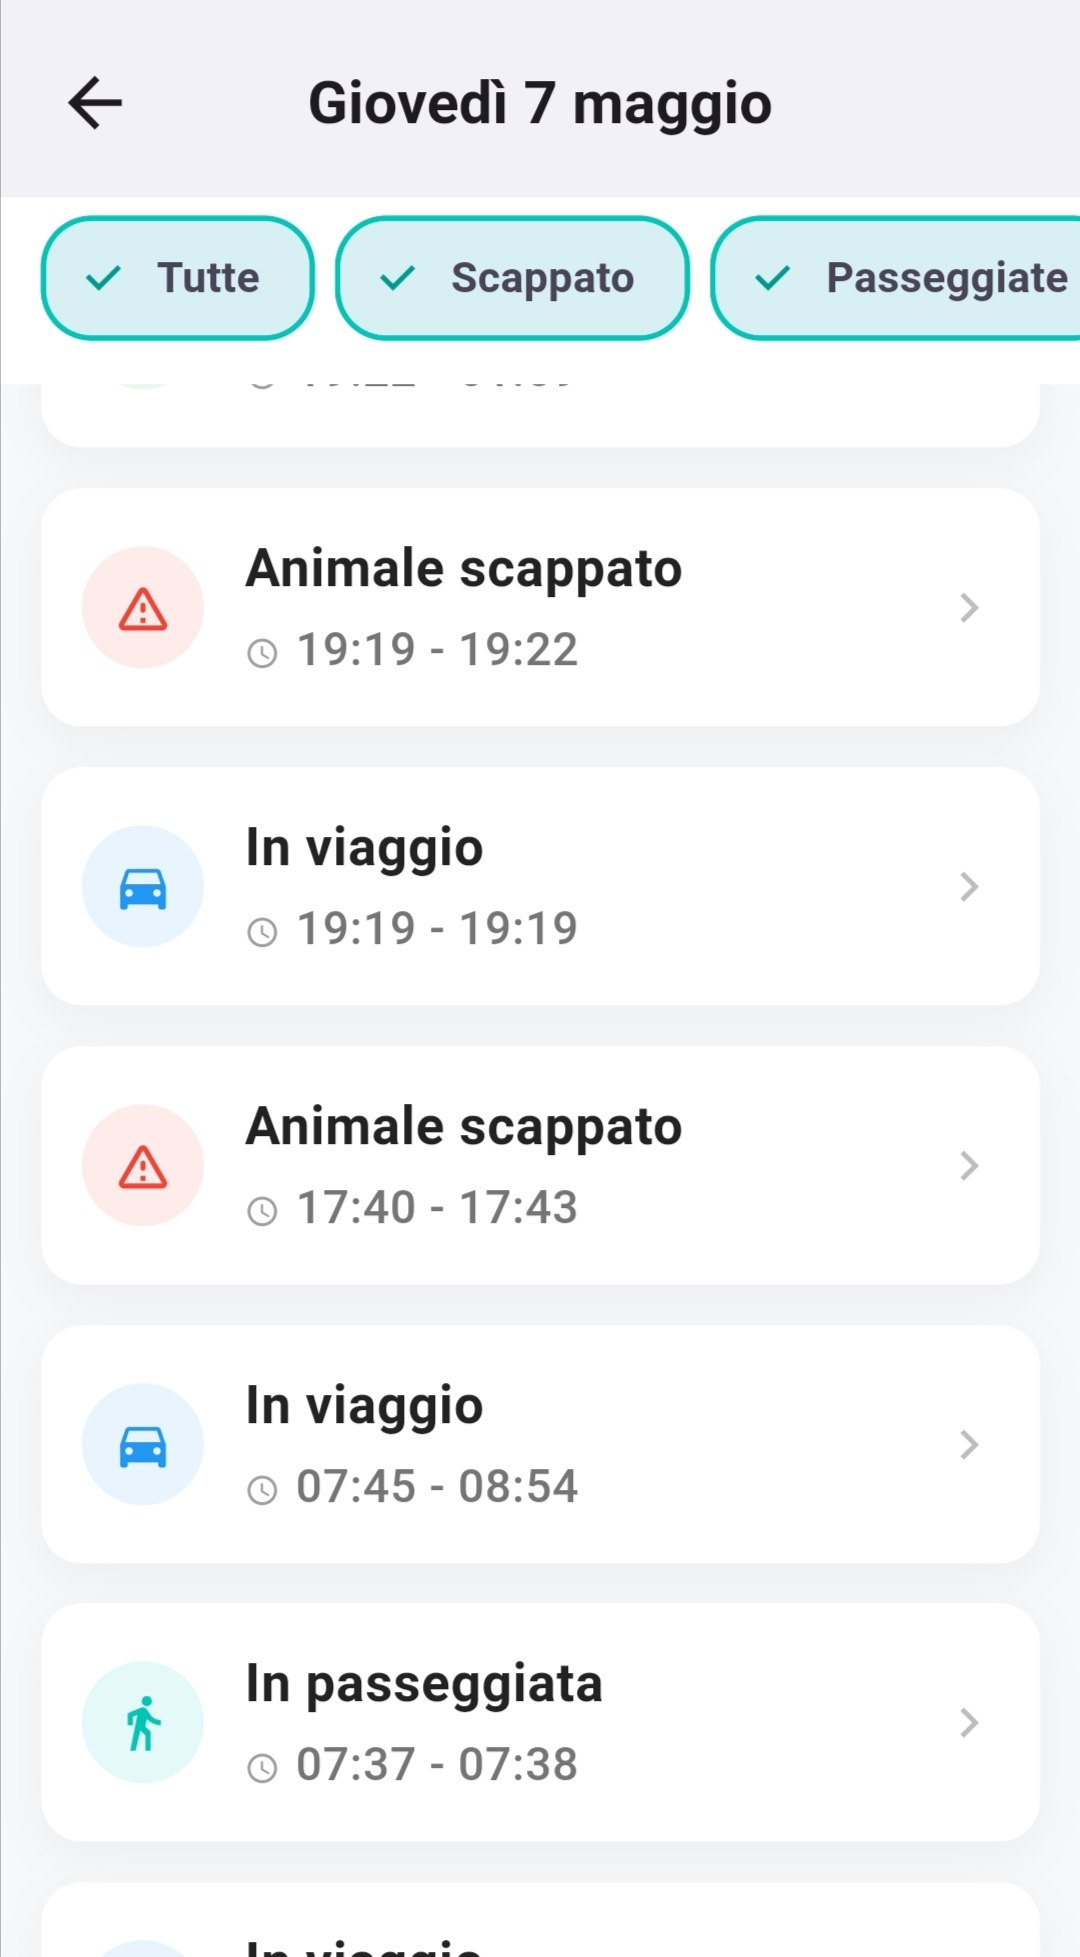
\includegraphics[width=\textwidth, height=8cm, keepaspectratio]{Immagini/Capitolo_5/photo_6.jpg}
        \caption{Visualizzazione di tutte le attività.}
        \label{fig:activity_list}
    \end{subfigure}
    \hfill 
    % Seconda immagine (Destra)
    \begin{subfigure}[b]{0.47\textwidth}
        \centering
        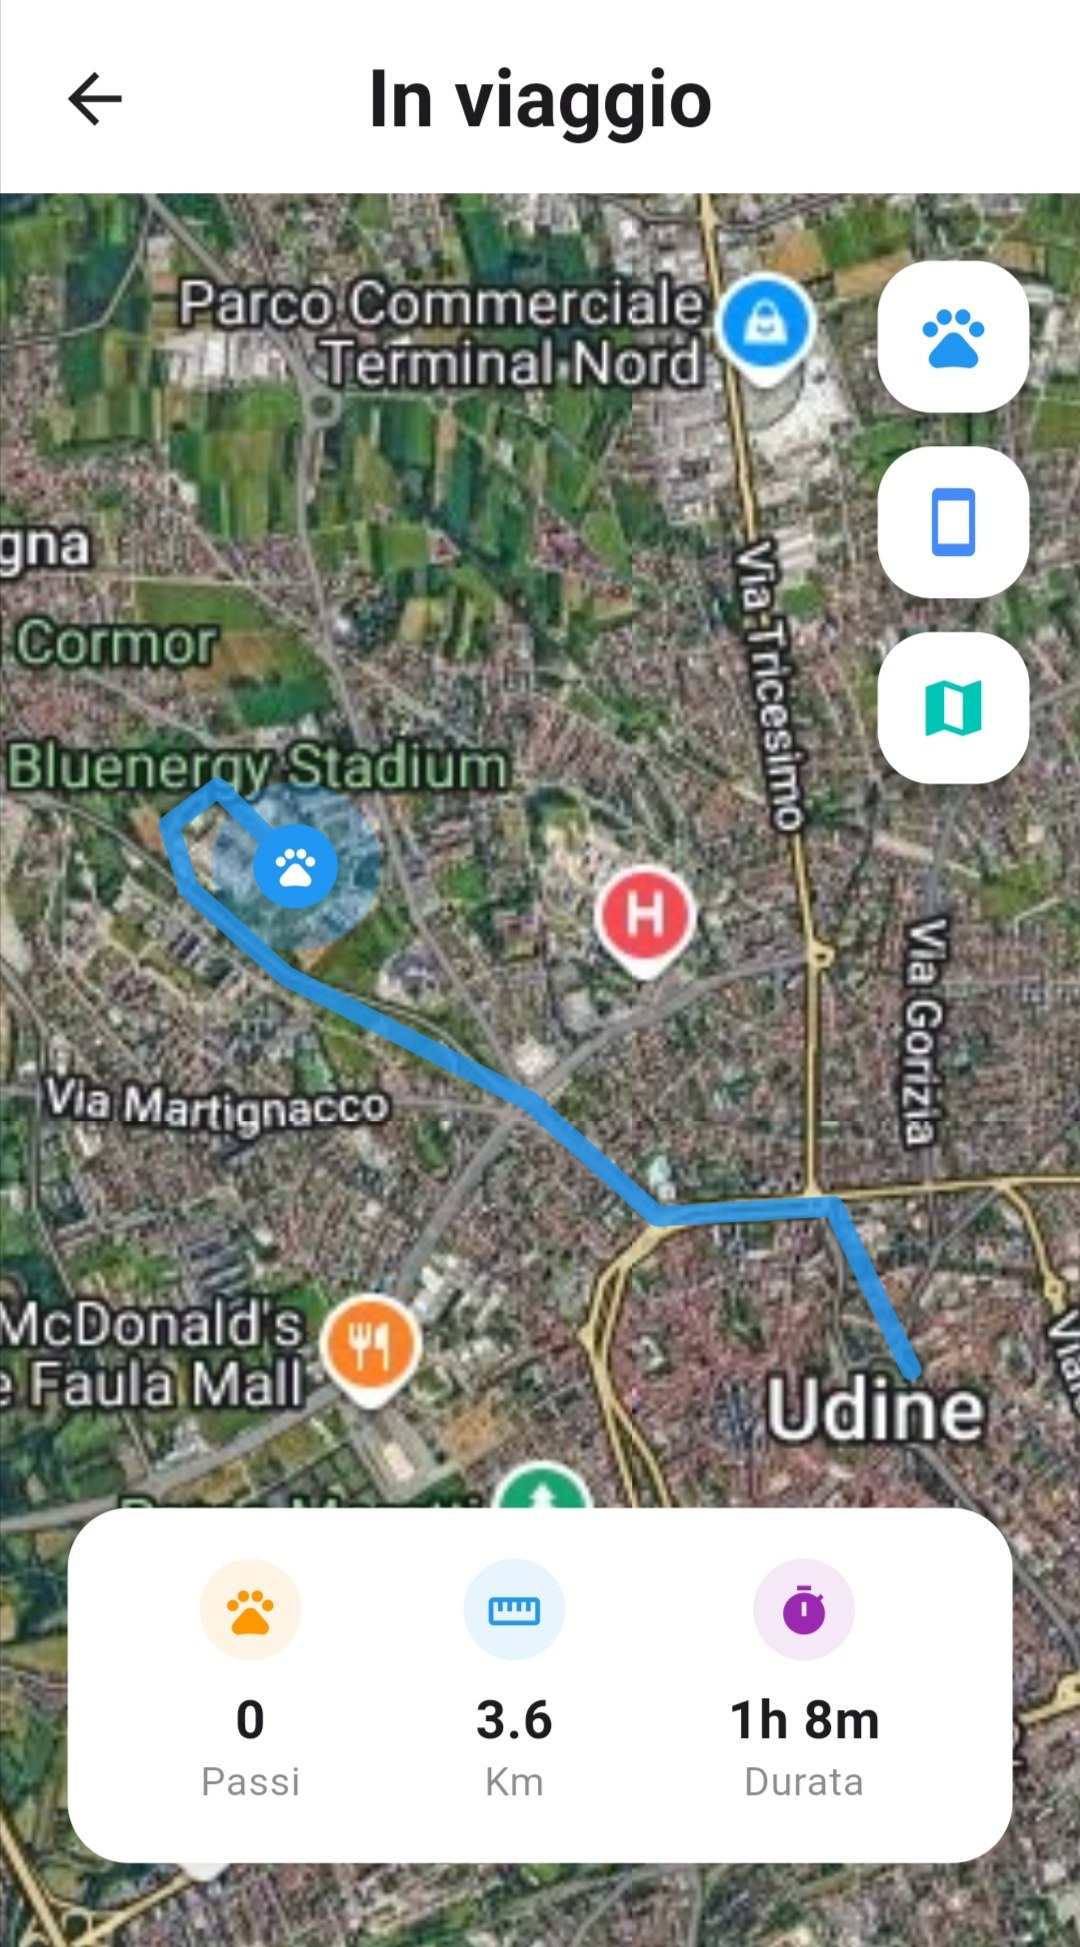
\includegraphics[width=\textwidth, height=8cm, keepaspectratio]{Immagini/Capitolo_5/photo_3.jpg}
        \caption{Dettagli di un'attività.}
        \label{fig:a_form}
    \end{subfigure}
\end{figure}

\subsubsection{Mappe in Tempo Reale}

L’app utilizza mappe interattive sviluppate con \texttt{flutter\_map}, 
permettendo di localizzare utente e animale in una visuale satellitare o stradale. 
La libreria viene ottimizzata tramite l'uso dei tile di \texttt{OpenStreetMap}, 
ovvero piccoli tasselli d'immagine caricati dinamicamente solo per l'area inquadrata, 
riducendo drasticamente il consumo di dati. 
Per preservare la batteria dello smartphone, 
le posizioni si aggiornano in tempo reale solo quando c'è un vero movimento, 
inoltre l'utente viene localizzato solo se ha dato il permesso.

Il sistema di controllo geografico si articola in due schermate principali 
che si scambiano dinamicamente in base allo stato dell'allarme. 
Quando l'allarme è disattivato, l'utente accede al sistema di \texttt{geofencing.dart}, 
un robusto strumento di sicurezza preventiva che permette di definire e gestire
i confini virtuali rappresentati come poligoni sulla mappa. 

All'attivazione dell'allarme, la schermata \texttt{geofencing.dart} passa a \texttt{tracking.dart}. 
In questa fase, il sistema adotta un approccio proattivo di sicurezza 
implementando un'interfaccia adattiva che cambia tra una modalità 
di monitoraggio e una di "inseguimento" qualora l’animale lasci la sua zona sicura attiva. 
Sulla mappa inoltre viene renderizzata una scia storica 
delle ultime posizioni registrate, fornendo un percorso visivo immediato 
che aiuta a comprendere la direzione del movimento recente dell’animale. 

\subsubsection{Gestione delle Zone Sicure}

Dopo l’inserimento di un indirizzo (manuale o GPS) o 
la selezione di una zona dalla pagina di geofencing,
la creazione e modifica delle aree avviene tramite \texttt{polygon\_editor.dart}.
L’utente può definire il perimetro toccando lo schermo per aggiungere i vertici.
L'interfaccia è progettata per essere estremamente flessibile, 
consentendo all'utente non solo di aggiungere o annullare i vertici, 
ma anche di rifinirne la forma trascinando i punti già posizionati.
Oltre a richiedere un minimo di tre vertici per formare una figura geometrica chiusa, 
un'area può essere creata solo se rispetta due controlli di validità:

\begin{itemize}
    \item Il \textbf{baricentro dell'area} non deve essere troppo distante dall'indirizzo selezionato, 
    impedendo così la creazione di zone a più di 50 metri dal segnaposto reale.
    \item Non deve esserci alcuna \textbf{sovrapposizione con zone già esistenti} al fine di garantire 
    l'univocità dei perimetri ed evitare conflitti logici durante il tracciamento.
\end{itemize}

\begin{figure}[htbp]
    \centering
    % Prima immagine (Sinistra)
    \begin{subfigure}[b]{0.31\textwidth}
        \centering
        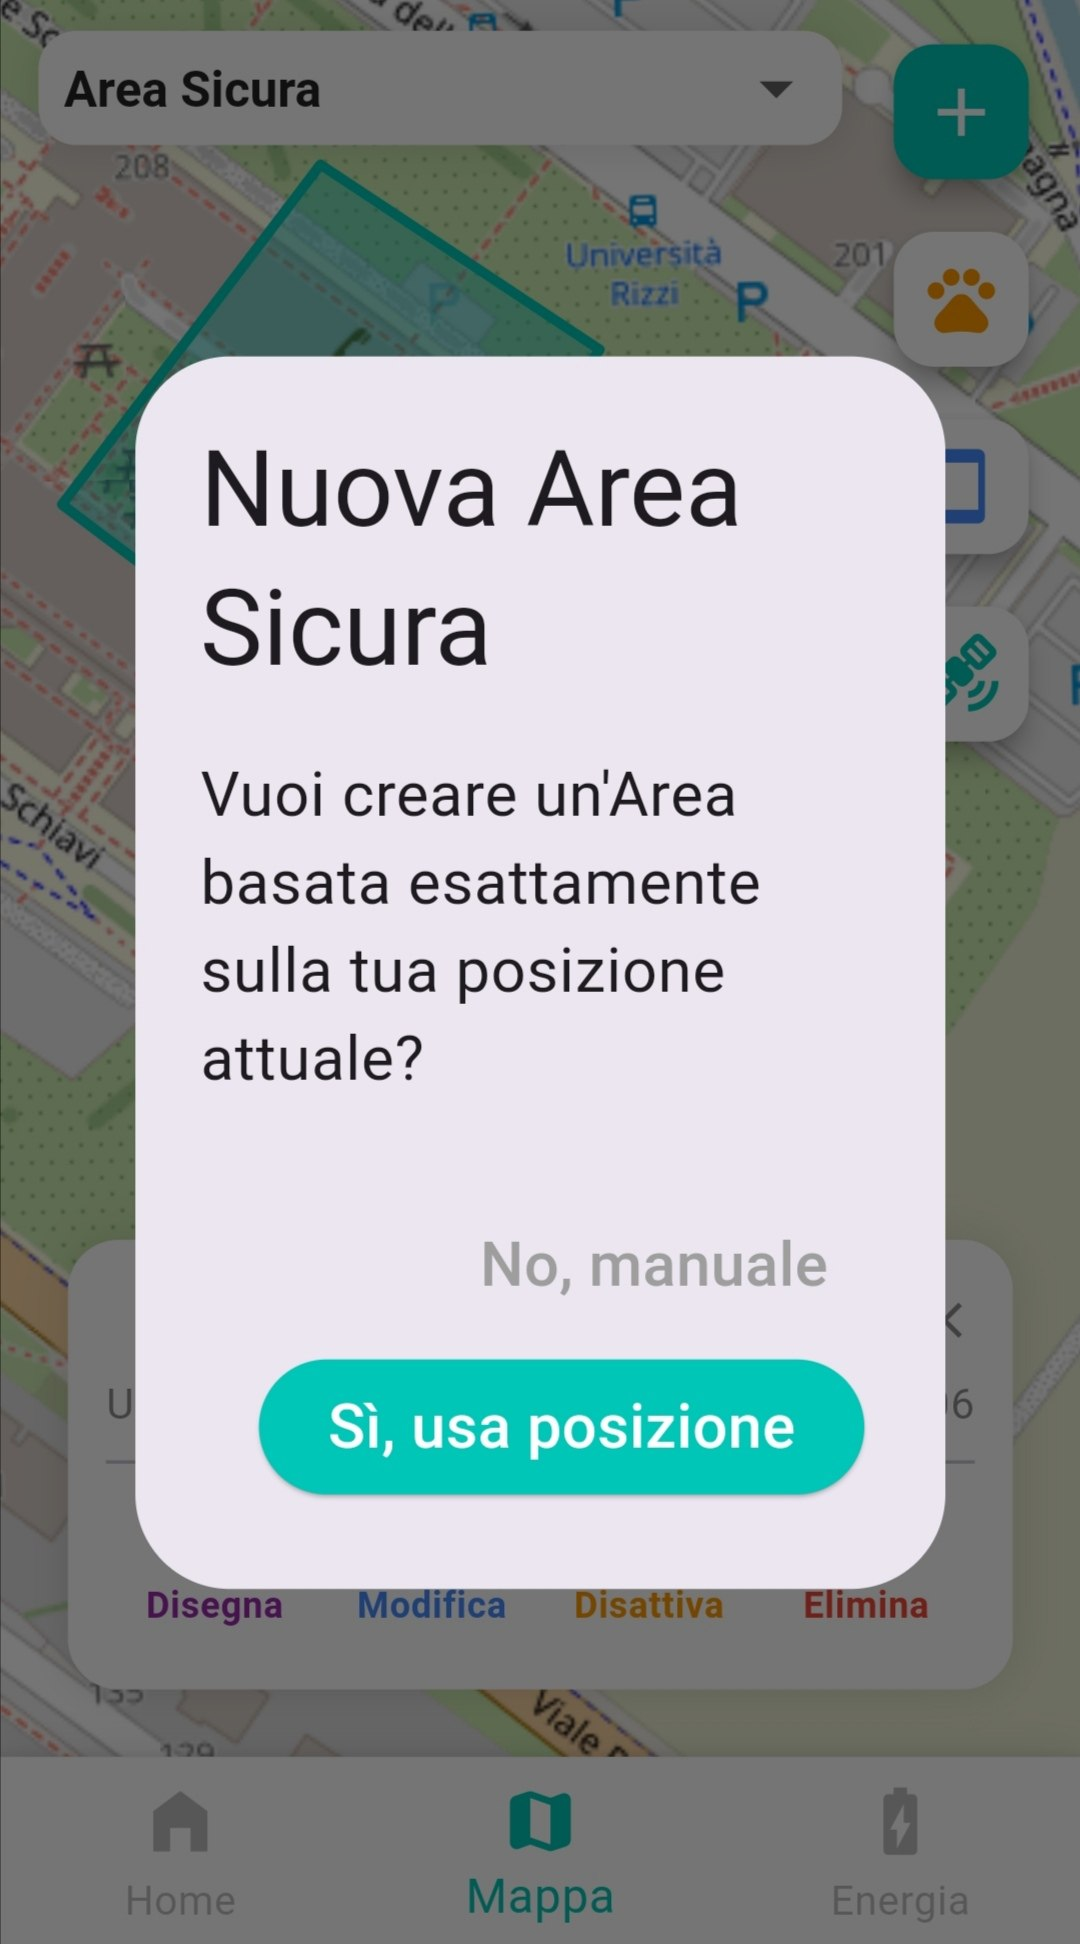
\includegraphics[width=\textwidth, height=8cm, keepaspectratio]{Immagini/Capitolo_5/photo_5.jpg}
        \caption{Scelta dell'inserimento.}
        \label{fig:area_choose}
    \end{subfigure}
    \hfill 
    % Seconda immagine (Centro)
    \begin{subfigure}[b]{0.31\textwidth}
        \centering
        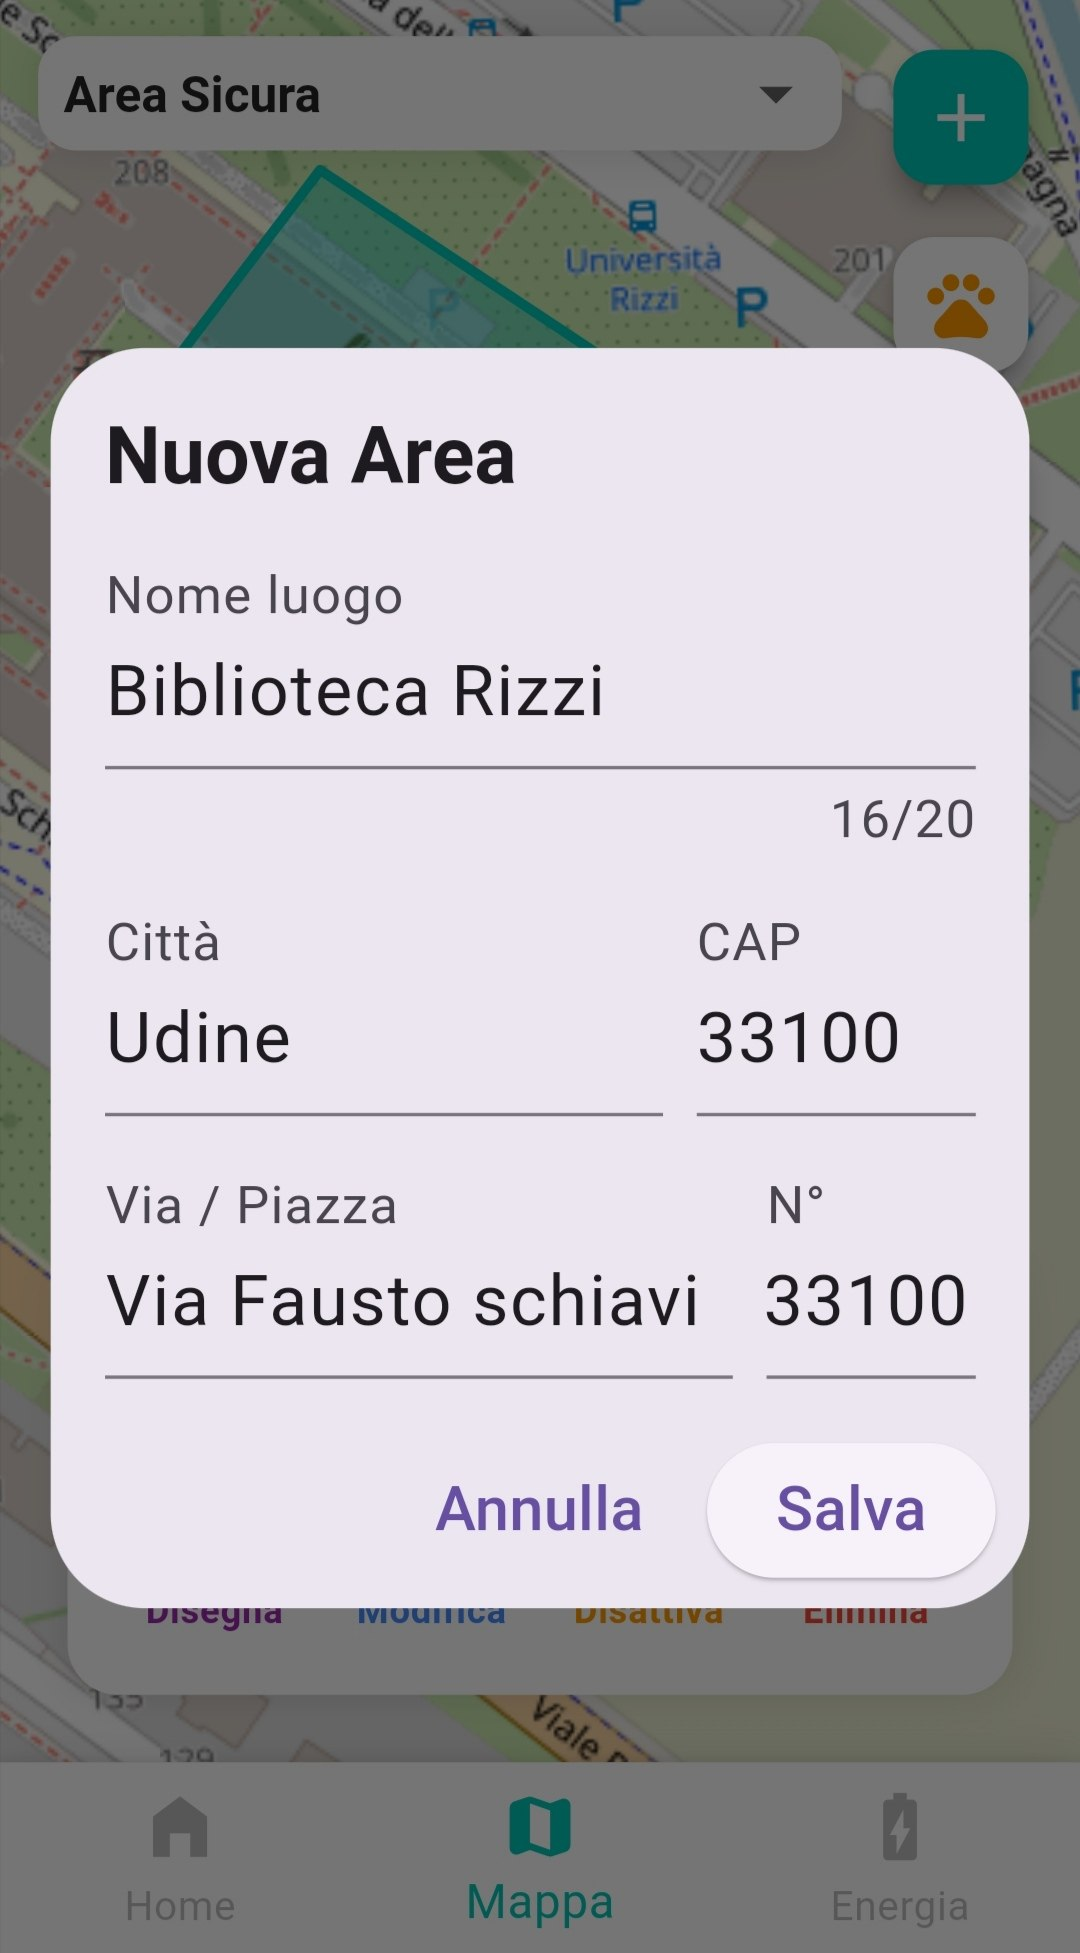
\includegraphics[width=\textwidth, height=8cm, keepaspectratio]{Immagini/Capitolo_5/photo_4.jpg}
        \caption{Compilazione indirizzo.}
        \label{fig:area_form}
    \end{subfigure}
    \hfill 
    % Terza immagine (Destra)
    \begin{subfigure}[b]{0.31\textwidth}
        \centering
        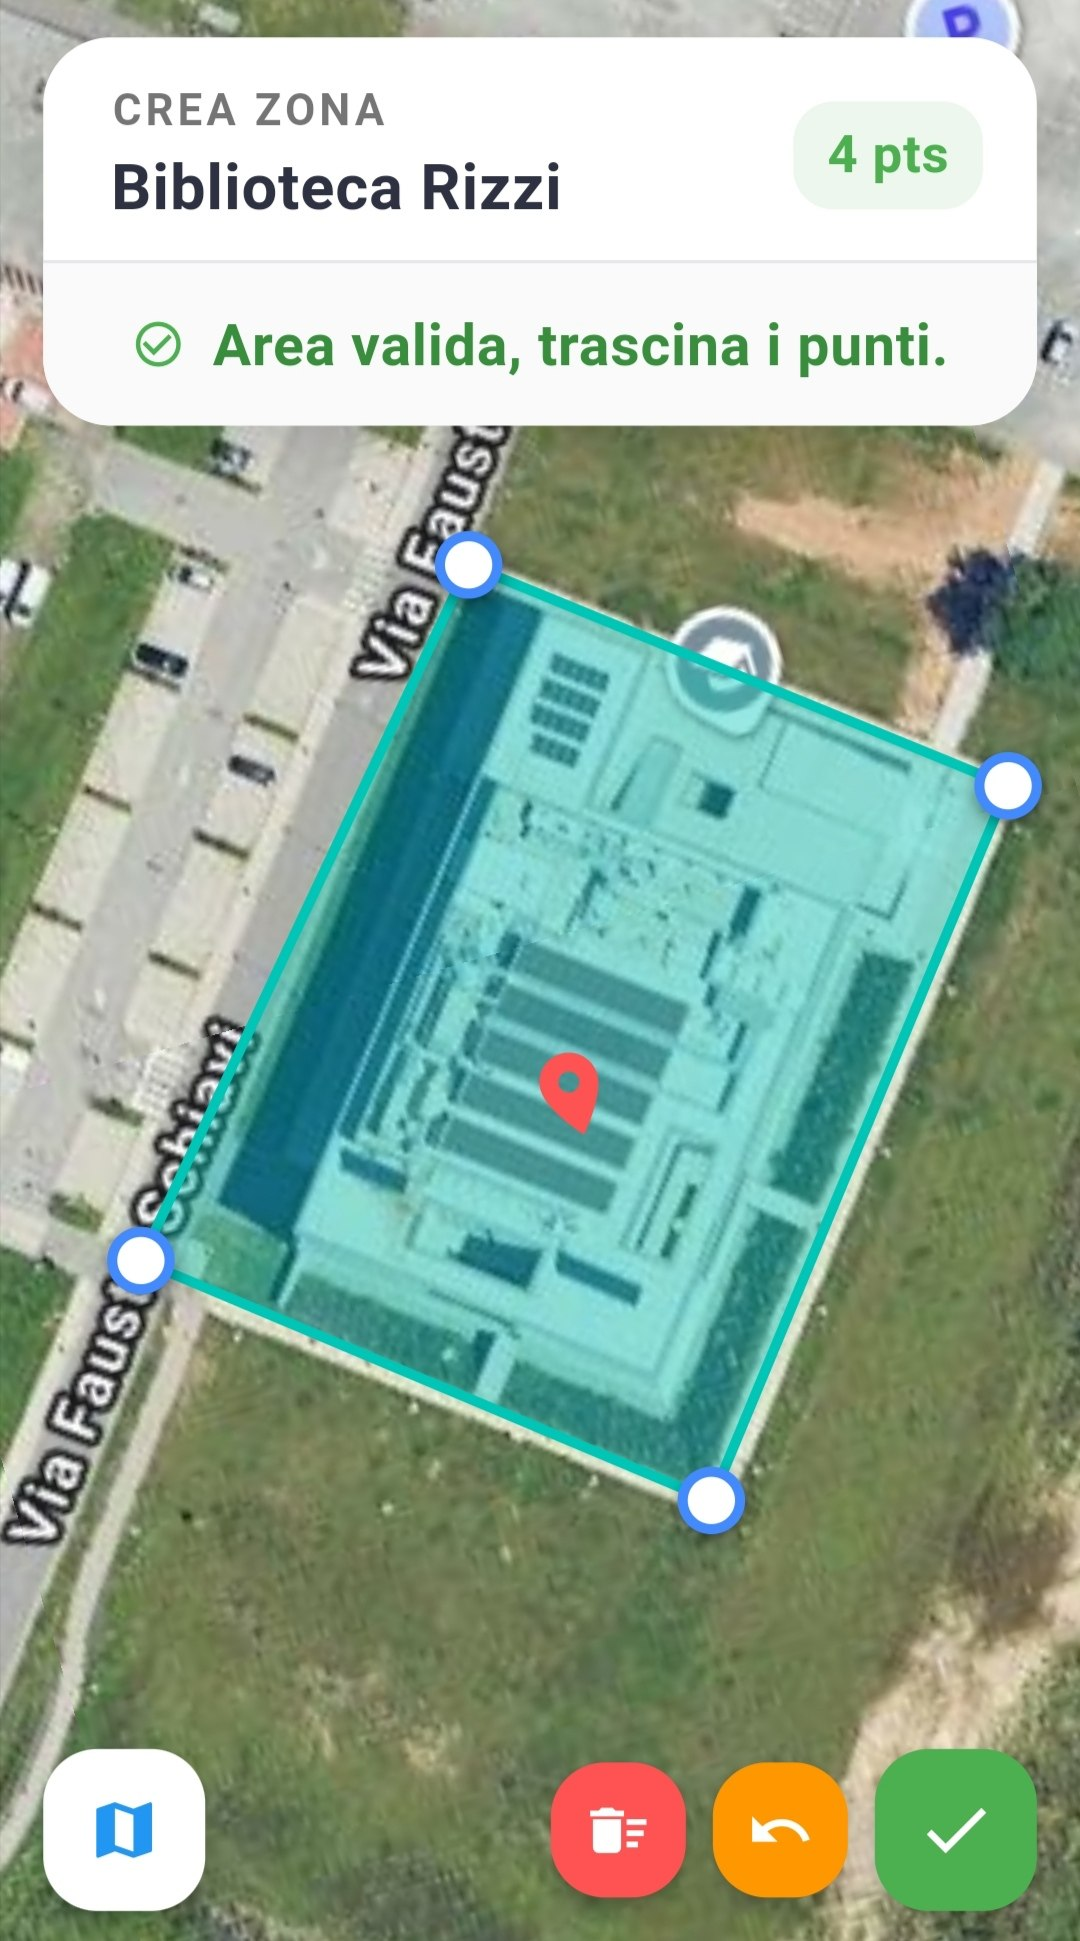
\includegraphics[width=\textwidth, height=8cm, keepaspectratio]{Immagini/Capitolo_5/photo_2.jpg}
        \caption{Disegno dell'area.}
        \label{fig:area_mappa}
    \end{subfigure}
    \label{fig:creazione_area}
\end{figure}

\section{Sistema di Notifiche Push}
L'implementazione di un sistema di notifiche push è fondamentale per un dispositivo di tracciamento animali, in quanto permette di avvisare tempestivamente l'utente in caso di pericoli (uscita dal perimetro sicuro) o problemi tecnici (batteria scarica).
\subsection{Analisi dei Vincoli Tecnologici: Incompatibilità Goja e Firebase}
Durante la fase di sviluppo, è emerso un vincolo tecnico significativo riguardante l'integrazione tra il backend PocketBase e l'SDK ufficiale di Firebase. 
PocketBase è scritto in linguaggio Go e utilizza \textbf{Goja} come motore di esecuzione JavaScript per la gestione della logica server-side (hooks). Goja è un'implementazione di ECMAScript 5.1 che presenta limitazioni strutturali rispetto a un ambiente Node.js \cite{nodejs} standard:
\begin{itemize}
    \item \textbf{Mancanza di moduli nativi}: Goja non supporta i moduli core di Node.js (come \texttt{fs}, \texttt{crypto} o \texttt{net}), indispensabili per il funzionamento dell'SDK di Firebase.
    \item \textbf{Runtime isolato}: L'SDK \texttt{firebase-admin} \cite{firebase_admin} richiede un ambiente di esecuzione completo per gestire l'autenticazione tramite Service Account e le connessioni persistenti ai server Google.
\end{itemize}
Per superare queste limitazioni, è stata adottata un'architettura a \textbf{Bridge}, separando la logica di business dall'invio fisico dei messaggi.
\subsection{Architettura del FCM Bridge}
Il sistema si basa su un microservizio esterno sviluppato in Node.js \cite{nodejs}, denominato \textit{FCM Bridge}. L'interazione avviene secondo il seguente flusso:
\begin{enumerate}
    \item \textbf{PocketBase (Goja)}: Rileva un evento (es. batteria scarica) e invia una richiesta HTTP POST al bridge tramite il modulo interno \texttt{\$http.send}.
    \item \textbf{FCM Bridge (Node.js)}: Riceve la richiesta, carica il Service Account di Firebase e inoltra la notifica tramite l'SDK ufficiale \cite{firebase_admin}.
    \item \textbf{Feedback e pulizia token}: Il bridge restituisce lo stato della consegna. In caso di errore \texttt{404} (token non registrato, app disinstallata) o \texttt{400} (token malformato), il backend provvede alla rimozione automatica del token dal profilo utente. I token FCM sono memorizzati come array JSON per supportare più dispositivi per singolo utente.
\end{enumerate}
\subsection{Logica di Invio e Trigger}
Le notifiche vengono scatenate dai seguenti eventi, ciascuno con logica contestuale per evitare invii ridondanti:

\begin{table}[H]
\centering
\begin{tabular}{@{}lp{4.5cm}p{5cm}@{}}
\toprule
\textbf{Evento} & \textbf{Condizione di trigger} & \textbf{Nota} \\
\midrule
Uscita dalla zona      & \texttt{i} $\to$ \texttt{s} oppure \texttt{i} $\to$ \texttt{w} & Dipende dalla presenza di allarme utente \\
Rientro in zona        & \texttt{s} $\to$ \texttt{i} oppure \texttt{w} $\to$ \texttt{i} & \\
Allarme da passeggiata & \texttt{w} $\to$ \texttt{s}                                    & Allarme riattivato mentre fuori zona \\
Inizio viaggio confermato & qualsiasi $\to$ \texttt{v/r}                     & Dipende dallo stato dell'allarme\\
Fine viaggio in zona   & \texttt{v/r} $\to$ \texttt{i}                                    & \\
Fine viaggio fuori zona (allarme) & \texttt{v/r} $\to$ \texttt{s}                        & \\
Fine viaggio fuori zona (libero)  & \texttt{v/r} $\to$ \texttt{w}                        & \\
Nessuna geofence       & \texttt{i} o \texttt{s} $\to$ \texttt{w}               & Zone disattivate \\
Batteria bassa         & $\leq 20\%$ (cambio soglia)                                    & Solo al cambio di fascia \\
Batteria critica       & $\leq 10\%$ (cambio soglia)                                    & Solo al cambio di fascia \\
Batteria in carica     & \texttt{charging} passa a \texttt{true}                        & Solo al cambio di stato \\
Watchdog               & Silenzio $>$ 10 minuti                                         & Chiusura automatica sessione \\
\bottomrule
\end{tabular}
\caption{Trigger del sistema di notifiche push}
\label{tab:notifiche}
\end{table}

\subsection{Gestione permessi}

Per abilitare la ricezione delle notifiche lato client, 
è stato fondamentale integrare 
il file di configurazione \texttt{google-services.json}, 
generato direttamente dalla console di Firebase 
e inserito all'interno della directory \texttt{android/app} del codice sorgente.
Questo file contiene le chiavi API, l'identificativo del progetto (\texttt{Project ID}) 
e i dettagli di configurazione necessari per autenticare in modo sicuro 
l'applicazione mobile con i servizi Google, 
senza esporre le credenziali nel codice in chiaro. 
Durante la fase di build, il \textit{plugin Gradle} di Google Services,
che si occupa di mappare i parametri di configurazione nel codice Android,
processa questo file per inizializzare automaticamente 
l'SDK di Firebase all'avvio dell'app,
abilitando così la connessione sicura a FCM 
e la generazione del token univoco del dispositivo.
Quest'ultimo viene dapprima salvato localmente 
e poi sincronizzato con il profilo utente su PocketBase 
all'interno del campo \texttt{tokenFCM}. 
Tale campo è modellato come una lista 
per permettere all'utente di ricevere le allerte 
su più dispositivi contemporaneamente; 
prima di ogni salvataggio, un controllo di duplicazione 
verifica che il \textit{token} non sia già presente, 
evitando così la ricezione di notifiche ridondanti.

\section{Vincoli di Sistema}
Nonostante i risultati ottenuti, il sistema presenta alcune limitazioni:
\begin{itemize}
    \item \textbf{Dipendenza dalla rete LTE}: senza copertura la trasmissione dati non è garantita.
    \item \textbf{Prestazioni indoor}: il modulo GNSS risulta poco affidabile in ambienti chiusi.
    \item \textbf{Backend locale}: l'utilizzo di PocketBase su macchina locale, 
        esposto tramite ngrok, introduce dipendenze da servizi esterni e limita la scalabilità.
    \item \textbf{Race condition sui pacchetti simultanei}: in caso di ricezione 
        quasi simultanea di due pacchetti dallo stesso dispositivo, 
        entrambi potrebbero leggere lo stesso record \texttt{activity} 
        prima del completamento della prima scrittura. 
        Gli scenari più critici sono due: 
        nel caso di cambio di stato, il secondo pacchetto potrebbe sovrascrivere 
        un record già chiuso dal primo, generando inconsistenze strutturali; 
        nel caso di risveglio simultaneo dal \textit{deep sleep}, 
        entrambi i pacchetti potrebbero riattivare 
        lo stesso record \texttt{sleep} e creare due sessioni attive 
        contemporaneamente, violando l'invariante del sistema. 
        L'impossibilità di gestire transazioni atomiche isolate 
        sui singoli record tramite le API standard di PocketBase 
        rende questo scenario non eliminabile lato applicativo. 
        Tuttavia, la frequenza di invio (ogni 30 o più secondi) 
        rende l’evento estremamente raro all'atto pratico.
    \item \textbf{Fallimento nella geolocalizzazione}: l'eventuale mancato rilevamento 
        di indirizzi, solitamente nei nei centri abitati più piccoli, 
        non è imputabile al codice, bensì a un limite legato alla densità dei metadati geografici. 
        Poiché \texttt{OpenStreetMap} si basa su contributi volontari, 
        l'assenza di tag specifici (come i numeri civici o il CAP associato alla via) 
        rende inefficaci le query strutturate inviate a \texttt{Nominatim}. 
        Quest'ultimo, richiedendo una corrispondenza rigida ed esatta di tutti i parametri forniti, 
        non è in grado di compensare l'incompletezza dei dati.
\end{itemize}

\section{Implementazioni Future}
Il progetto nel suo percorso di sviluppo ha trovato delle possibiità future di scalabilità dell'App, di seguito le idee che abbiamo accavallato per procedere nella migliore implementazione delle precedenti funzioni descritte.

\subsection{Stato della batteria}
Per garantire all'utente un corretto valore della batteria aggiornato sugli ultimi pacchetti è richiesto un calcolo con dati storici, questo è uno dei possibili ulteriori passaggi che può essere sviluppato all'interno dell'applicazione per quanto riguarda i dati da fornire all'utente. Non risulta come attività critica in quanto il sistema riesce a garantire all'utente una notifica nel momento in cui la batteria raggiunge (e scende) sotto il livello del 20\%.

\subsection{Database, Infrastruttura Cloud e Gestione della Concorrenza}
Il passaggio da un ambiente di prototipazione locale a una soluzione orientata alla produzione prevede la migrazione dell'intero backend su un'infrastruttura Cloud dedicata (PaaS o VPS come AWS, Google Cloud o DigitalOcean). Questa evoluzione consentirà di superare i vincoli attuali attraverso i seguenti interventi strutturali:
\begin{itemize}
    \item \textbf{Assegnazione di Dominio e Sicurezza TLS:} Sostituendo il tunnel temporaneo \texttt{ngrok} con un dominio di secondo livello proprietario, protetto da certificati SSL/TLS (es. Let's Encrypt), si garantirà una connessione HTTPS/WSS nativa, stabile e priva di interruzioni di sessione o rate-limiting arbitrari.
    \item \textbf{Risoluzione delle Race Condition via Message Broker:} Per azzerare il rischio di collisione nell'aggiornamento simultaneo delle attività (derivante dalla ricezione di pacchetti ravvicinati), si prevede l'introduzione di un middleware di messaggistica asincrona, come \texttt{Redis} o \texttt{RabbitMQ}, interposto tra l'endpoint di ricezione e il database. Questo livello fungerà da coda FIFO (\textit{First-In, First-Out}), serializzando i pacchetti provenienti dallo stesso tracker ed eseguendo le transazioni in modo strettamente sequenziale, preservando così l'invariante del sistema.
    \item \textbf{Migrazione del DBMS:} Qualora il volume di dispositivi connessi dovesse saturare le capacità di lock di SQLite, l'architettura consentirà di scalare verticalmente migrando verso un database relazionale centralizzato (come \texttt{PostgreSQL}), nativamente ottimizzato per transazioni ACID altamente concorrenti.
\end{itemize}

\subsection{Ingegnerizzazione e Costruzione della Scheda Hardware}
L'attuale prototipo hardware, sebbene funzionale alla validazione del software, richiede una fase di ingegnerizzazione elettronica per poter essere trasformato in un dispositivo commerciale realmente indossabile dall'animale. Lo sviluppo futuro si articolerà su tre assi principali:
\begin{itemize}
    \item \textbf{Sviluppo di un PCB Custom:} Progettazione di un circuito stampato personalizzato (\textit{Printed Circuit Board}) mediante strumenti EDA (come KiCad o Altium Designer). L'integrazione del microcontrollore, del modem LTE e del modulo GNSS su un'unica scheda consentirà di ridurre drasticamente il fattore di forma (\textit{form factor}), minimizzando l'ingombro e il peso del tracker sul collare dell'animale.
    \item \textbf{Ottimizzazione del Power Management:} Introduzione di un circuito integrato dedicato alla gestione dell'energia (\textit{PMIC}) e di un chip di \textit{fuel gauge} hardware (es. serie MAX17043). Questo permetterà di implementare il calcolo predittivo basato sui dati storici menzionato nella sezione precedente, offrendo letture della percentuale di carica estremamente precise e non inficiate dai picchi di assorbimento del modem durante la trasmissione.
    \item \textbf{Industrial Design e Protezione Ambientale:} Progettazione di un \textit{enclosure} (involucro) personalizzato tramite modellazione 3D e stampaggio a iniezione. La scocca dovrà garantire un grado di protezione minimo pari a \textbf{IP67} o \textbf{IP68}, rendendo il dispositivo totalmente impermeabile all'acqua, al fango e resistente agli urti causati dai movimenti repentini dell'animale all'aperto.
\end{itemize}

\section{Conclusioni}

\newpage

\addcontentsline{toc}{section}{Riferimenti bibliografici}
\printbibliography[title={Riferimenti bibliografici}]

\end{document}